\chapter{E2E Test Framework}
\label{chap:e2e-test-framework}

\section{Automated E2E Testing}
\label{sec:automated-e2e-testing}

\subsection{Manual vs Automatic E2E Testing}
\label{sec:manual-vs-automatic-e2e-testing}

The advantages of automated testing versus manual testing become apparent when considering the complexity of handling all possible test cases, their results and how to mitigate application build issues based on the test results.
\\

Manual testing requires the use of a table of test cases which needs to be administered by a human. It is not efficient as it takes a long time to go through, especially if there are a large number of test cases. The overhead of administrative work necessary for updating the table with results slows down the development process and shifts the focus towards less critical work.
\\

The situation worsens as complexity grows because of the need to test on multiple browsers and against multiple builds which may differ in any number of ways.
\\

We can solve many of these problems using automation. In automated E2E testing, a program can be written which can:

\begin{itemize}
\item Allow human readable test scenarios (BDD)
\item Open a browser and execute the scenarios
\item Record the results and any issues
\item Insert and clear data associated with test cases
\end{itemize}

\begin{center}
\begin{longtable}{ |p{3.7cm}|p{4.6cm}|p{4.6cm}| }
 \hline
 	\multicolumn{3}{|c|}{Comparison of Manual and Automated Testing} \\
 \hline
 	& \multicolumn{1}{|c|}{Manual Testing} & \multicolumn{1}{|c|}{Automatic Testing} \\
 \hline
 	Test Accuracy & Prone to human error. & More reliable as it is performed by automation tools.\\
 \hline
    Time Consuming & Time consuming, taking up human resources. & Generally faster than manual testing but with a considerable amount of test cases it can also take long.\\
 \hline
    Practicality & Not practical with a large number of test cases or when frequent repetition is required. & Practical option when the test cases are run repeatedly over a long period of time.\\
 \hline
    Results Accuracy & Gives low accuracy results. & Gives high accuracy results.\\
 \hline
    Human Observation & Human observation is part of the testing process and easier to reason about the results. & No human observation as tests are run via automated scripts.\\
 \hline
    Cost effectiveness & Costs less because fewer tools are needed but the cost of human resources makes it an expensive practice. & Expensive due to tool costs but can be mitigated by using open-source software. Less budget needed for human resources.\\
 \hline
    Results visibility & More insight when executing tests because of human observation but less overview on general testing outcome. & No insight while executing the automated tests but a good overview of testing outcomes due to reporting tools.\\
 \hline
 \caption{Manual Testing vs. Automatic Testing}
 \label{tab:manual-vs-automatic}
\end{longtable}
\end{center}

\vspace{-1.5cm}

\section{Technologies Used}
\label{sec:technologies-used}

\subsection{Selenium}
\label{subsec:selenium}
The \textit{Selenium WebDriver} is an open-source software that interacts directly with the browser. It can be used to automate browser interactions such as clicking buttons, scrolling up and down a page, accessing specific URLs and much more.
\\

The \textit{Selenium WebDriver} operates via a server that takes incoming requests via an API. The server translates these into asynchronous commands which communicate with the browser driver.
\\

Many APIs have been written to work with \textit{Selenium} so it can be used with a multitude of languages including JavaScript. It is compatible with the majority of BDD and TDD testing frameworks. For our project we used the \texttt{webdriver-manager} \texttt{Node} module which is embedded within the \textit{Protractor} framework.

\subsection{Protractor}
\label{subsec:protractor}
\textit{Protractor} is an E2E test framework for \textit{AngularJS} applications. It can be combined with a number of TDD/BDD test frameworks such as \textit{Jasmine}, \textit{Mocha} and \textit{Cucumber}. \textit{Protractor} works in conjunction with \textit{Selenium} to provide an automated test infrastructure that can simulate a user’s interaction with an \textit{Angular} application running in a browser or a mobile device.
\\

The role of \textit{Protractor} is essentially of a wrapper around \textit{Selenium WebDriver} to better suit \textit{AngularJS} applications. It gets rid of the overhead of managing asynchronous calls and blends nicely the nature of JavaScript with the particularities of \textit{Selenium}.

\subsection{Cucumber}
\label{subsec:cucumber}
\textit{Cucumber} is an open-source BDD testing framework used to add business level logic to automated testing. It has a number of different implementations for a variety of languages.
\\

As explained in \textbf{Section \ref{subsubsec:bdd}}, BDD allows for a certain layering of abstraction levels to satisfy both non-technical and technical people. It defines its formal requirements in feature files which contain test scenarios that the related feature should be able to offer. These files can document all the necessary functionality of a particular application. The business level language used in feature files is called \textit{Gherkin}. Each action in a scenario is called a \texttt{step} and each \texttt{step} has an underlying implementation provided by a \texttt{step} function.
\\

\textit{Cucumber} sits on top of \textit{Protractor}, offering a convenient BDD environment best suited for \textit{AngularJS} applications.

\section{Test Framework Components}
\label{sec:test-framework-components}

\subsection{Requirements as Feature Definitions}
\label{subsec:feautre-definition-as-requirements}

Feature files can be seen as an entry point to \textit{Cucumber} test cases \cite{featurefile1}. Each of the feature files should be written to test a single feature of the application or a particular area of the feature \cite{featurefile2}. Since we were writing E2E tests for the payment feature, we created \texttt{buycredits.feature} file for testing this aspect. Consider \textbf{Listing \ref{lst:buycredits-feature-file}}:\\

\begin{listing}[H]
\begin{minted}[xleftmargin=\parindent, linenos, breaklines, breakanywhere, bgcolor=lightgray, fontsize=\small]{cucumber}
@dev @experiment
Feature: Buying Credit feature
  As a user of Synote
  I should be able to successfully buy credits when logged in

  Scenario: Access buy credits page when logged in
    Given I click the "Profile" button on "SideMenu" page
    Given I click the "BuyCredit" button on "Profile" page
    Then I should be on "BuyCredits" page

  Scenario: Buy credit with empty card number
    Given I click the "Profile" button on "SideMenu" page
    Given I click the "BuyCredit" button on "Profile" page
    Given I Correctly type in my details but "" for "number"
    Then Submit button should be disabled
# code omitted
\end{minted}
\captionof{listing}{\texttt{Buying Credit Feature} Test Cases}
\label{lst:buycredits-feature-file}
\end{listing}

The section in \textbf{Listing \ref{lst:buycredits-feature-file}} is written in a language called \textit{Gherkin}. \textit{Gherkin} makes use of Business Readable Domain Specific Language (BRDSL) which allows us to write the test cases at a business level without getting into implementation details.\\

Our client required us to document the specification for the new payment feature. Since most of Synote's team are developers and the feature file used \textit{Gherkin}, it was readable on a business level and could act as an automation test script \cite{featurefile1}. Hence, we recommended using the feature files themselves as the requirements documentation.\\

Each of the feature files should be defined with the \texttt{Feature} keyword which consists of a name  (see \textbf{Listing \ref{lst:buycredits-feature-file}} line  2) and a brief description  (see \textbf{Listing \ref{lst:buycredits-feature-file}} line  3-4). Each of the test cases are defined with the \texttt{Scenario} keyword followed by a brief description of that test (see \textbf{Listing \ref{lst:buycredits-feature-file}} line  6 and 11). Each scenario should \cite{featurefile3}:
\begin{itemize}
\item Describe the event taking place
\item Describe the expected result
\end{itemize}

We use \texttt{Steps} to achieve this. Consider the \texttt{Access buy credits page when logged in} scenario in \textbf{Listing \ref{lst:buycredits-feature-file}}. We use keywords such as \texttt{Given} (line 7 and 8) and \texttt{Then} (line 9) for writing readable test cases. Consider \textbf{Table \ref{tab:steps-keywords}} which define \texttt{Step} keywords \cite{featurefile1}:

\begin{center}
%Column widths dependent on page width/margins
\begin{tabular}{ |p{2cm}|p{7cm}| }

 \hline
 	\multicolumn{1}{|c|}{Keyword} &
 	\multicolumn{1}{|c|}{Description}\\
 \hline
 	Given & Describes test pre-condition\\
 \hline
 	And & Defines additional test conditions\\
 \hline
 	Then & Defines expectations of test \\
 \hline

\end{tabular}
\captionof{table}{\texttt{Step Keywords}}
\label{tab:steps-keywords}
\end{center}

\vspace{-1cm}
\subsection{Reusable Steps Definition}
\label{subsec:reusable-steps-definition}

\textit{Cucumber} is not able to execute the scenarios as they are. Instead, we have to write \texttt{step} definitions. \texttt{Step} definitions use regular expression to map the \textit{Gherkin} \texttt{steps} to actions which will drive system interactions \cite{stepfile1}. Each of the \texttt{steps} written for \texttt{scenario}s in the \texttt{feature} file should have a \texttt{step} definition declared in its corresponding \texttt{step} file. A \texttt{step} file should only contain definitions for \texttt{steps} used in the corresponding \texttt{feature} file. Consider \textbf{Listing \ref{lst:buycredits-step-file}}:\\

\begin{listing}[H]
\begin{minted}[xleftmargin=\parindent, linenos, breaklines, breakanywhere, bgcolor=lightgray, fontsize=\small]{js}
//code omitted
this.Given(/^I click the "([^"]*)" button on "([^"]*)" page$/,
  function (buttonName, pageName) {
    return this.Support.clickButton(buttonName, pageName);
});

this.Given(/^I should be on "([^"]*)" page$/, function (pageName) {
  return this.Support.waitUntil
      (this.Support.urlChanged(this.Support.getPageUrl(pageName))
    , 2000)();
});
//code omitted
\end{minted}
\captionof{listing}{\texttt{Step} Definitions for \texttt{Access buy credits page when logged in scenario}}
\label{lst:buycredits-step-file}
\end{listing}

All the \texttt{steps} written in the \texttt{buycredits.feature} file are defined in the \texttt{buycredits.steps.js} file. Each step should have a unique definition, otherwise an \texttt{ambiguous match exception} will be thrown. \textbf{Listing \ref{lst:buycredits-step-file}} contains the \texttt{step} definitions for \texttt{Access buy credits page when logged in} scenario in \textbf{Listing \ref{lst:buycredits-feature-file}}. Inside the \texttt{step} definitions, we write JavaScript code to handle the interaction logic e.g. 1st definition in \textbf{Listing \ref{lst:buycredits-step-file}} (line 2) handles clicking of button, given the \texttt{buttonName} and \texttt{pageName} parameters. The 2nd definition (line 7) checks that we are on a page with the correct URL associated with the \texttt{pageName} parameter. Nearly all of our \texttt{step} definitions take parameters instead of hard-coding them. This way, we can satisfy the DRY principle by reusing generic \texttt{step} definitions, making both  \texttt{feature} and  \texttt{step} files easily maintainable and readable.

\subsection{Reusable Support Functions}
\label{subsec:reusable-support-functions}

In order to have generic \texttt{step} definitions (see \textbf{Listing \ref{lst:buycredits-step-file}} line 3 and 7), we needed to write common generic methods which will drive interactions with the system. We place such functions in the \texttt{support.js} file. As a rule of thumb, we identified generic methods to go in the \texttt{support.js} file by checking if we were repeating any code/logic in the \texttt{buycredits.steps.js} file. Currently, our framework uses the \texttt{support.js} file for:

\begin{itemize}
\item Clicking
\item Filling inputs
\item Navigating
\item Data retrieval
\end{itemize}

\begin{listing}[H]
\begin{minted}[xleftmargin=\parindent, linenos, breaklines, breakanywhere, bgcolor=lightgray, fontsize=\small]{js}
//code omitted
function loadPageOnSupport(pageName) {
  if (!support[pageName]) {
    support[pageName] = require
      ('../pages/' + pageName.toLowerCase() + '.page.js');
  }
}
//code omitted
fillInputOnPage: function (pageName, textBox, text) {
  loadPageOnSupport(pageName);
  if (this[pageName] && this[pageName][textBox + 'Input']) {
    var _textBox = this[pageName][textBox + 'Input'];
    return _textBox.sendKeys(text);
  }
}
//code omitted
\end{minted}
\captionof{listing}{\texttt{loadPageOnSupport} and \texttt{fillInputOnPage} Support Functions }
\label{lst:support-file-methods}
\end{listing}

Consider \textbf{Listing \ref{lst:support-file-methods}}. \texttt{fillInputOnPage} is a common generic method i.e. it can be used to fill any input field on any page, hence its placement in the \texttt{support.js} file. The \texttt{loadPageOnSupport} method helps \texttt{support.js} file to be generic in applying its methods in different contexts by dynamically requiring desired pages objects. The main advantage of \texttt{support.js} is that testers will never have to rewrite any code they have already written which satisfies the DRY principle.

\subsection{Pre and Post Hooks}
\label{subsec:pre-and-post-hooks}

Hooks are snippets of code that can be executed before or after individual test scenarios (\textit{Cucumber} hooks) or the entire test suite (\textit{Protractor} hooks). We use them for a variety of purposes.

\subsubsection{Data Insertion and Clearing}
\label{subsubsec:data-insertion-and-clearing}
In order to enforce the SILO principle such that each test scenario is independent of other scenarios, we clear any previous data related to a case that might have existed before and then we insert the information that we need.\\

The way we accomplish this is by sending a POST request to the Synote server telling it what data we need. The server will then parse the incoming request and add the required data to the database. This is done via the \texttt{setupTestData} method in \texttt{support.js} which constructs the request with the given arguments and sends it to the server to be parsed. This can be seen below:

\begin{listing}[H]
\begin{minted}[xleftmargin=\parindent, linenos, breaklines, breakanywhere, bgcolor=lightgray, fontsize=\small]{js}
setupTestData : function (argArr) {
  return httpPost('Testing/setup', argArr);
}
\end{minted}
\captionof{listing}{Method in \texttt{support.js} for inserting test data}
\label{lst:inserting-test-data}
\end{listing}

The process of specifying what data to add is wrapped around a \textit{Cucumber} \texttt{step} function which describes the application's pre-existing state that is needed. For example, the scenario below requires that the user already has a card saved with some specific details.

\begin{listing}[H]
\begin{minted}[xleftmargin=\parindent, linenos, breaklines, breakanywhere, bgcolor=lightgray, fontsize=\small]{cucumber}
Scenario: Pay with saved card
  Given I already have a card saved with correct details except "4242424242424242,7,2017,123" for "number,exp_month,exp_year,cvc"
  Given I click the "Profile" button on "SideMenu" page
  Given I click the "BuyCredit" button on "Profile" page
  Then "PaySavedRadio" Button on "BuyCredits" page should be visible
  Given I click card at position "1" on BuyCredits page
  And I click the "SubmitPayment" button on "BuyCredits" page
  Then  I should be on "CreditsHistory" page
\end{minted}
\captionof{listing}{Example scenario with DB setup}
\label{lst:example-scenario-with-db-setup}
\end{listing}

The highlighted step will map to the function below which will send the arguments to the Synote server.

\begin{listing}[H]
\begin{minted}[xleftmargin=\parindent, linenos, breaklines, breakanywhere, bgcolor=lightgray, fontsize=\small]{js}
this.Given(/^I already have a card saved with correct details except "([^"]*)" for "([^"]*)"$/,
  function (value, fieldName) {
    var tempCard = this.Support.getEnvFieldCustom("defaultCard",
      this._.zipObject(this._.split(fieldName, ','),
      this._.split(value, ',')));
    delete tempCard['billing_name'];
    tempCard['exp_month'] = this.
      BuyCreditsPage.convertMonthNameToNumber(tempCard['exp_month']);

    return this.Support.setupTestData({
      steps : 'saveCard',
      params : {
        card : tempCard
      },
      email : browser.deployment.defaultUser.email
    });
});
\end{minted}
\captionof{listing}{Data insertion \texttt{step} function}
\label{lst:data-insertion-step-function}
\end{listing}

All the test data related to a user is cleared out before each \texttt{scenario} and each test run which enforces the SILO principle.

\begin{listing}[H]
\begin{minted}[xleftmargin=\parindent, linenos, breaklines, breakanywhere, bgcolor=lightgray, fontsize=\small]{js}
this.Before(function () {
  return this.Support.cleanTestData
          (browser.deployment.defaultUser.email);
});
\end{minted}
\captionof{listing}{Remove test data before scenario}
\label{lst:remove-test-data-before-scenario}
\end{listing}

\subsubsection{Login and Logout}
\label{subsubsec:login-and-logout}

\textit{Cucumber} hooks can also be used for authenticating users. Currently we login before each test scenario and logout afterwards. This can be seen on the listing \textbf{Listing \ref{lst:login-and-logout-hooks}}:

\begin{listing}[H]
\begin{minted}[xleftmargin=\parindent, linenos, breaklines, breakanywhere, bgcolor=lightgray, fontsize=\small]{js}

this.Before(function () {
  this.Support.fillInputOnPage(this.LoginPage.Title, "Email", browser.deployment.defaultUser.email);

  this.Support.fillInputOnPage(this.LoginPage.Title, "Password", browser.deployment.defaultUser.password);

  return this.Support
    .clickButton("Login", this.LoginPage.Title)
    .then(this.Support.waitUntil(this.Support.urlChanged
          (browser.deployment.hostUrl)
        , 2000));
});

this.After(function () {
  return this.Support
    .clickButton("Logout", this.HeaderPage.Title)
    .then(this.Support.waitUntil(this.Support.urlChanged
          (this.Support.getPageUrl(this.LoginPage.Title))
        , 2000));
});

\end{minted}
\captionof{listing}{Login and logout hooks}
\label{lst:login-and-logout-hooks}
\end{listing}

In the future, an enhancement would be to add \textit{Cucumber} tags to the \texttt{scenario}s that require logging in specifically as opposed to doing it all the time.

\subsubsection{User locking and unlocking}
\label{subsubsec:user-locking-and-unlocking}

A problematic context is when multiple people are using the framework at the same time and running tests on the same deployment with the same user test accounts. We envisioned this might cause issues. To deal with it, we created a pool of user accounts. This is represented by a database table on the server which contains all the user test accounts along with a flag for each. The flag says whether or not the account in question is locked for testing or not. The account is locked once the test suite begins executing and is then unlocked at the end.
\\

This is done via HTTP \texttt{POST} requests to the Synote server. When locking a user, the framework demands a user of a particular type. If all the accounts of that type are locked, an informative error is thrown. Methods in \texttt{support.js} handle sending the HTTP requests as seen in \textbf{Listing \ref{lst:lock-and-unlock-users}}:

\begin{listing}[H]
\begin{minted}[xleftmargin=\parindent, linenos, breaklines, breakanywhere, bgcolor=lightgray, fontsize=\small]{js}
lockUser : function (role) {
  return httpPost('Testing/lock', {
    role : role
  });
},

unlockUser : function (email) {
  return httpPost('Testing/unlock', {
    email : email
  });
}
\end{minted}
\captionof{listing}{Lock and Unlock Users}
\label{lst:lock-and-unlock-users}
\end{listing}

\subsection{Page Objects}
\label{subsec:page-objects}
There are few key interactions which are very common throughout the application e.g. clicking buttons, filling inputs, navigating pages etc. It seemed tedious and time consuming to actually write separate methods for these interactions on different pages. We came to the conclusion that the interactions themselves should be generic enough so they can be applied to any page. The pages of the application differed in the elements and components they had. Hence, we have definitions of \texttt{Page Object Models} which are composed of a page's elements.\\

The \texttt{buycredits.html} page (\textbf{Figure \ref{fig:paymentform-screenshot}}) and it's corresponding \texttt{page object file} (\textbf{Listing \ref{lst:buycredits-page-code}}) create  a one to one mapping of the page components. Page object files also house methods to interact with elements (defined in the same \textit{page object model}) which are only applicable to the particular page in question e.g. \texttt{buycreditspage.js} has a method called \texttt{fillDefaultCardDetails} which fills in the payment form fields and is only applicable to \texttt{buycredits.html} page. The main advantages of implementing page objects are reduced code duplication and easy maintainability i.e.  if any of the UI elements of the application were changed, we only have to modify them in the page object file instead of fixing them in each \texttt{step} which used that UI element \cite{semaphore}. Another advantage is that it structures the framework, making it more readable.

\begin{minipage}{.48\textwidth}
\begin{listing}[H]
\begin{minted}[xleftmargin=\parindent, linenos, breaklines, breakanywhere, bgcolor=lightgray, fontsize=\small]{js}
{ // buyCredits.page.js snippet
Title : "BuyCredits",
Url : browser.deployment.hostUrl + 'buycredit',

billing_nameInput : element
  (by.model('billingName')),

numberInput : element
  (by.model('cardNumber')),

cvcInput : element
  (by.model('cardCVC')),

exp_monthInput : element
  (by.model('expMonth')),

exp_yearInput : element
  (by.model('expYear')),

PaySavedRadioButton : element
  (by.id('pay-saved-radio')),
//code omitted
}
\end{minted}
\captionof{listing}{Element Mappings for Payment Form}
\label{lst:buycredits-page-code}
\end{listing}
\vspace{0.1cm}
\end{minipage}%
\begin{minipage}{.49\textwidth}
  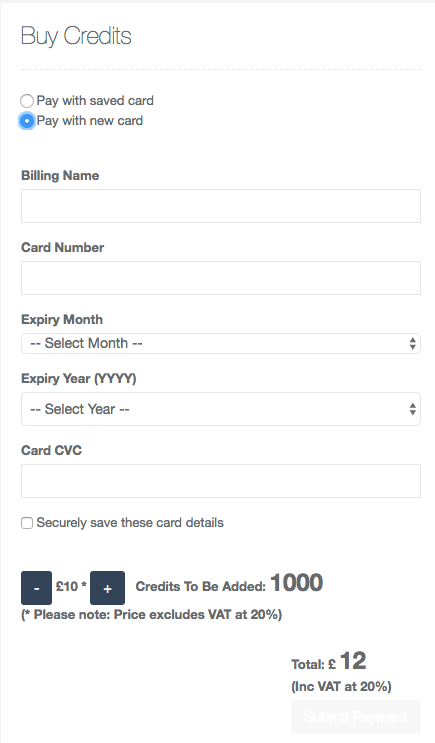
\includegraphics[width=\textwidth]{screenshot-payment-form.png}
  \captionof{figure}{Payment Form}
 	\label{fig:paymentform-screenshot}
\end{minipage}

\subsection{Deployment Definition}
\label{subsec:deployment-definition}
One of the requirements of our client was that our framework should be capable of running the E2E test suite against different deployments of Synote application. The main concern we had here was that tests which worked on one deployment may not work on another deployment because each deployment of Synote uses different parameters. For example host URI of \texttt{development} deployment is \url{http://localhost:9000/\#/} and for  \texttt{experiment} deployment, it is \url{https://experiment.synote.com/\#/}. Same with other parameters such as cards e.g. \texttt{development} should use test card whereas live deployments such as \texttt{production} should use live cards. It can be very time consuming to manually enter all this data when you want to test a deployment. Thus we created \texttt{deployment.js} file which can be used to easily define different deployments of the Synote application.

\begin{listing}[H]
\begin{minted}[xleftmargin=\parindent, linenos, breaklines, breakanywhere, bgcolor=lightgray, fontsize=\small]{js}
//code omitted
deployment_name : { // e.g. experiment
  hostUrl : 'deployment_url', // e.g. https://experiment.synote.com
  apiEndpoint : 'backend_rest_api_url',
  defaultUser: {
    password : 'password',
    role: 'test_user_role'
  },
  defaultCard: {
    // test card for dev, real card for staging etc.
  }
}
//code omitted
\end{minted}
\captionof{listing}{Deployment Parameter Example}
\label{lst:deployment-file}
\end{listing}

Consider \textbf{Listing \ref{lst:deployment-file}}. Here you can see that each deployment of Synote is defined by different parameters. This way, we only have to define deployment specific data once for running the tests.

\begin{listing}[H]
\begin{minted}[xleftmargin=\parindent, linenos, breaklines, breakanywhere, bgcolor=lightgray, fontsize=\small]{bash}
	conf.js --params.env dev --cucumberOpts.tgs=@deployment_name
\end{minted}
\captionof{listing}{Running the E2E Tests}
\label{lst:specifying-deployment-test-run}
\end{listing}

When running the E2E tests, we simply need to pass the name of object which represents the deployment we want to test against. For example: consider \textbf{Listing \ref{lst:specifying-deployment-test-run}}, here we pass in \texttt{dev} as a parameter so the framework will execute tests on the \texttt{development} deployment with data defined in \texttt{dev} object.  To overcome the issues with some tests only being suitable for certain deployments, we used \textit{Cucumber tags} which can be placed on the \texttt{feature} keyword of the \texttt{feature} files or on the desired \texttt{scenarios}. For example, in \textbf{Listing \ref{lst:buycredits-feature-file}} we place \texttt{dev} and \texttt{experiment} keywords on the \texttt{feature} keyword so all the test \texttt{scenarios} will run for both of these deployments. The desired test suite to be executed has to be specified as a parameter when executing the tests (see \textbf{Listing \ref{lst:specifying-deployment-test-run}}).

\subsection{Example Test Case}
\label{subsec:example-test-case}

When testing a feature of the application, we initially start with a requirement which will later form the description of the \texttt{feature file}. For example, we want to test the \texttt{payment feature} and our requirement is \texttt{As a user of Synote I should be able to successfully buy credits when logged in}. First we will need to create a \texttt{feature} file as in \textbf{Listing \ref{lst:example-feature-file}}.

\begin{listing}[H]
\begin{minted}[xleftmargin=\parindent, linenos, breaklines, breakanywhere, bgcolor=lightgray, fontsize=\small]{cucumber}
Feature: Buying Credit feature
  As a user of Synote
  I should be able to successfully buy credits when logged in
\end{minted}
\captionof{listing}{Example \texttt{feature} Definition for Payment System}
\label{lst:example-feature-file}
\end{listing}

In \textbf{Listing \ref{lst:example-feature-file}} we use the \texttt{feature} keyword to title the feature under test i.e. \texttt{payment feature} and describe it via the requirement. The requirement is then broken down into sub-requirements which will together satisfy the main requirement. The sub-requirements are written as \texttt{scenarios}. Let a sub-requirement be \texttt{Buy credit with valid card details}. Then its corresponding \texttt{scenario} will look like:

\begin{listing}[H]
\begin{minted}[xleftmargin=\parindent, linenos, breaklines, breakanywhere, bgcolor=lightgray, fontsize=\small]{cucumber}
# code omitted
Scenario: Buy credit with valid card details
  Given I click the "Profile" button on "SideMenu" page
  Given I click the "BuyCredit" button on "Profile" page
  Given I Correctly type in my details
  And I click the "SubmitPayment" button on "BuyCredits" page
  Then I should be on "CreditsHistory" page
\end{minted}
\captionof{listing}{Example \texttt{Feature} File}
\label{lst:example-feature-file-scenario}
\end{listing}

In \textbf{Listing \ref{lst:example-feature-file-scenario}}, we have labelled the \texttt{scenario} with the sub-requirement definition itself and wrote \texttt{steps} in \textit{Gherkin} for testing it. If any of the \texttt{steps} take parameters, we specify them with quotes.\\

Next we need to create a \texttt{steps} file where \texttt{step} definitions for the 5 steps in \textbf{Listing \ref{lst:example-feature-file-scenario}} will be written. Consider \textbf{Listing \ref{lst:example-steps-file}}.

\begin{listing}[H]
\begin{minted}[xleftmargin=\parindent, linenos, breaklines, breakanywhere, bgcolor=lightgray, fontsize=\small]{js}
module.exports = function () {
  this.Given(/^I click the "([^"]*)" button on "([^"]*)" page$/,
    function (buttonName, pageName) {
      // write a generic method
  });
  this.Given(/^I Correctly type in my details$/, {timeout: 60*1000},
    function () {
      // write a page specific method for buy credits page
  });
  this.Given(/^I should be on "([^"]*)" page$/,
    function (pageName) {
      //write a generic method;
  });
}
\end{minted}
\captionof{listing}{Example \texttt{Steps File}}
\label{lst:example-steps-file}
\end{listing}

In \textbf{Listing \ref{lst:example-steps-file}} we define the \texttt{steps} written in \textbf{Listing \ref{lst:example-feature-file-scenario}} using reqular expressions. The \texttt{scenario} in \textbf{Listing \ref{lst:example-feature-file-scenario}} will be interacting with the payment form (see \textbf{Figure \ref{fig:paymentform-screenshot}}) and so we need to create a \texttt{page object file} for it as defined in  \textbf{Section \ref{subsec:page-objects}}.

\begin{listing}[H]
\begin{minted}[xleftmargin=\parindent, linenos, breaklines, breakanywhere, bgcolor=lightgray, fontsize=\small]{js}
var buyCreditsPage = {
  Title : "BuyCredits",
  Url : browser.deployment.hostUrl + 'buycredit',
  billing_nameInput : element(by.model('billingName')),
  numberInput : element(by.model('cardNumber')),
  cvcInput : element(by.model('cardCVC'))
  //code omitted
}
\end{minted}
\captionof{listing}{Example \texttt{Page Object} File}
\label{lst:example-page-file}
\end{listing}

In \textbf{Listing \ref{lst:example-page-file}}, we created a one to one mapping of all the elements of the payment form. Next step is to actually write interaction code to complete the \texttt{step} definitions in \textbf{Listing \ref{lst:example-steps-file}} using the page object.\\

Consider the 1st \texttt{step} definition in \textbf{Listing \ref{lst:example-steps-file}}. This can be grouped as a generic \texttt{step} since it can be applicable to many elements on different pages. Therefore we should create a generic method in \texttt{support.js} file for this interaction as mentioned in  \textbf{Section \ref{subsec:reusable-support-functions}}.

\begin{listing}[H]
\begin{minted}[xleftmargin=\parindent, linenos, breaklines, breakanywhere, bgcolor=lightgray, fontsize=\small]{js}
clickButton: function (buttonName, pageName) {
  loadPageOnSupport(pageName);
  var button = support.getButton(buttonName, pageName);
  return button.click();
},
\end{minted}
\captionof{listing}{Example Support Function for clicking}
\label{lst:example-support-func}
\end{listing}

\textbf{Listing \ref{lst:example-support-func}} shows a section of the \texttt{support} file with the generic method to handle clicking. See \textbf{Listing \ref{lst:example-step-def-click-completed}} to see usage of this function in the step definition.

\begin{listing}[H]
\begin{minted}[xleftmargin=\parindent, linenos, breaklines, breakanywhere, bgcolor=lightgray, fontsize=\small]{js}
//code omitted
this.Given(/^I click the "([^"]*)" button on "([^"]*)" page$/,
  function (buttonName, pageName) {
    return this.Support.clickButton(buttonName, pageName);
});
//code omitted
\end{minted}
\captionof{listing}{Completed Step Definition For Clicking Buttons}
\label{lst:example-step-def-click-completed}
\end{listing}

Now consider the 2nd \texttt{step} definition in \textbf{Listing \ref{lst:example-steps-file}}. This \texttt{step} is specific to the payment form only. Hence this interaction should be handled in the \texttt{page object} file for payment form.

\begin{listing}[H]
\begin{minted}[xleftmargin=\parindent, linenos, breaklines, breakanywhere, bgcolor=lightgray, fontsize=\small]{js}
//code omitted
fillInputsOnPage : function (pageName, fieldValMap){
  loadPageOnSupport(pageName);
  if (support[pageName]) {
    var promises = [];
    // enter the exception fields
    _.forOwn(fieldValMap, function (val, field) {
      if (field && val) {
        promises.push(support.fillInputOnPage(pageName, field, val));
      }
    });
    return Promise.all(promises);
  }
}
//code omitted
\end{minted}
\captionof{listing}{Payment Form Page Specific Method for Filling in Fields}
\label{lst:example-page-specific-method}
\end{listing}

\textbf{Listing \ref{lst:example-page-specific-method}} shows a section of the \texttt{page} file with an implementation of the method to fill inputs of payment form. See \textbf{Listing \ref{lst:example-step-def-fillin-completed}} to see usage of this function in the \texttt{step} definition.

\begin{listing}[H]
\begin{minted}[xleftmargin=\parindent, linenos, breaklines, breakanywhere, bgcolor=lightgray, fontsize=\small]{js}
//code omitted
this.Given(/^I Correctly type in my details$/, {timeout: 60*1000},
  function () {
    return this.BuyCreditsPage.fillDefaultCardDetails();
});
//code omitted
\end{minted}
\captionof{listing}{Completed Step Definition For Filling in Payment Form}
\label{lst:example-step-def-fillin-completed}
\end{listing}

Finally, consider the 3rd \texttt{step} definition in \textbf{Listing \ref{lst:example-steps-file}}. This can also be grouped as a generic \texttt{step} since it is applicable to different pages. Here we need to create the following methods in the \texttt{support} file for:

\begin{itemize}
\item Waiting a certain time for page to load
\item Checking current URL matches passed in URL
\end{itemize}

\begin{listing}[H]
\begin{minted}[xleftmargin=\parindent, linenos, breaklines, breakanywhere, bgcolor=lightgray, fontsize=\small]{js}
waitUntil : function (action, time) {
  return function () {
    return browser.wait(action, time);
  }
},
urlChanged : function(url) {
  return function () {
    return browser.getCurrentUrl().then(function(actualUrl) {
      return actualUrl === url;
    });
  };
}
\end{minted}
\captionof{listing}{Example Support Function For Checking Page URL}
\label{lst:example-support-func2}
\end{listing}

\textbf{Listing \ref{lst:example-support-func2}} shows implementation of generic methods required to complete the final step definition. See \textbf{Listing \ref{lst:example-step-def-url-check-completed}} to see usage of these functions in the step definition.

\begin{listing}[H]
\begin{minted}[xleftmargin=\parindent, linenos, breaklines, breakanywhere, bgcolor=lightgray, fontsize=\small]{js}
//code omitted
this.Given(/^I should be on "([^"]*)" page$/, function (pageName) {
  return this.Support.waitUntil
      (this.Support.urlChanged(this.Support.getPageUrl(pageName))
    , 2000)();
});
//code omitted
\end{minted}
\captionof{listing}{Completed Step Definition For Verifying Current URL}
\label{lst:example-step-def-url-check-completed}
\end{listing}

\subsection{Reporting}
\label{subsec:reporting}

Reporting is a very important part of the E2E testing framework. It should allow us to have a clear overview of what went wrong during tests, the state of the application and aid us in debugging issues.

\subsubsection{Types of Reporting}
\label{subsubsec:types-of-reporting}

Reporting for the E2E test results is of 3 types:

\begin{enumerate}

\item \textbf{Pretty printing in the console}
\\
This can be seen in \textbf{Figure \ref{fig:e2e-test-cases}}. It is mainly helpful for doing development as it offers a fast way of checking test results and debugging issues with stack traces.

\item \textbf{JSON reporting}
\\
This type of reporting is mainly used as a means of saving test results to file. It is what the majority of HTML reporting software uses as input.

\item \textbf{HTML reporting}
\\
The \textit{Node} module that we used for reporting is \texttt{cucumber-html-report}. You can see a screenshot of an example report in \textbf{Figure \ref{fig:html-report-example}}. We chose it mainly because:

\begin{itemize}
\item It has a nice outline that allows you to navigate rapidly between test cases and scenarios
\item Colour coding makes it easy to read
\item Good debugging power as it shows you the stack trace of the failed tests
\end{itemize}

\end{enumerate}

\begin{figure}[!hbt]
  	\centering
 	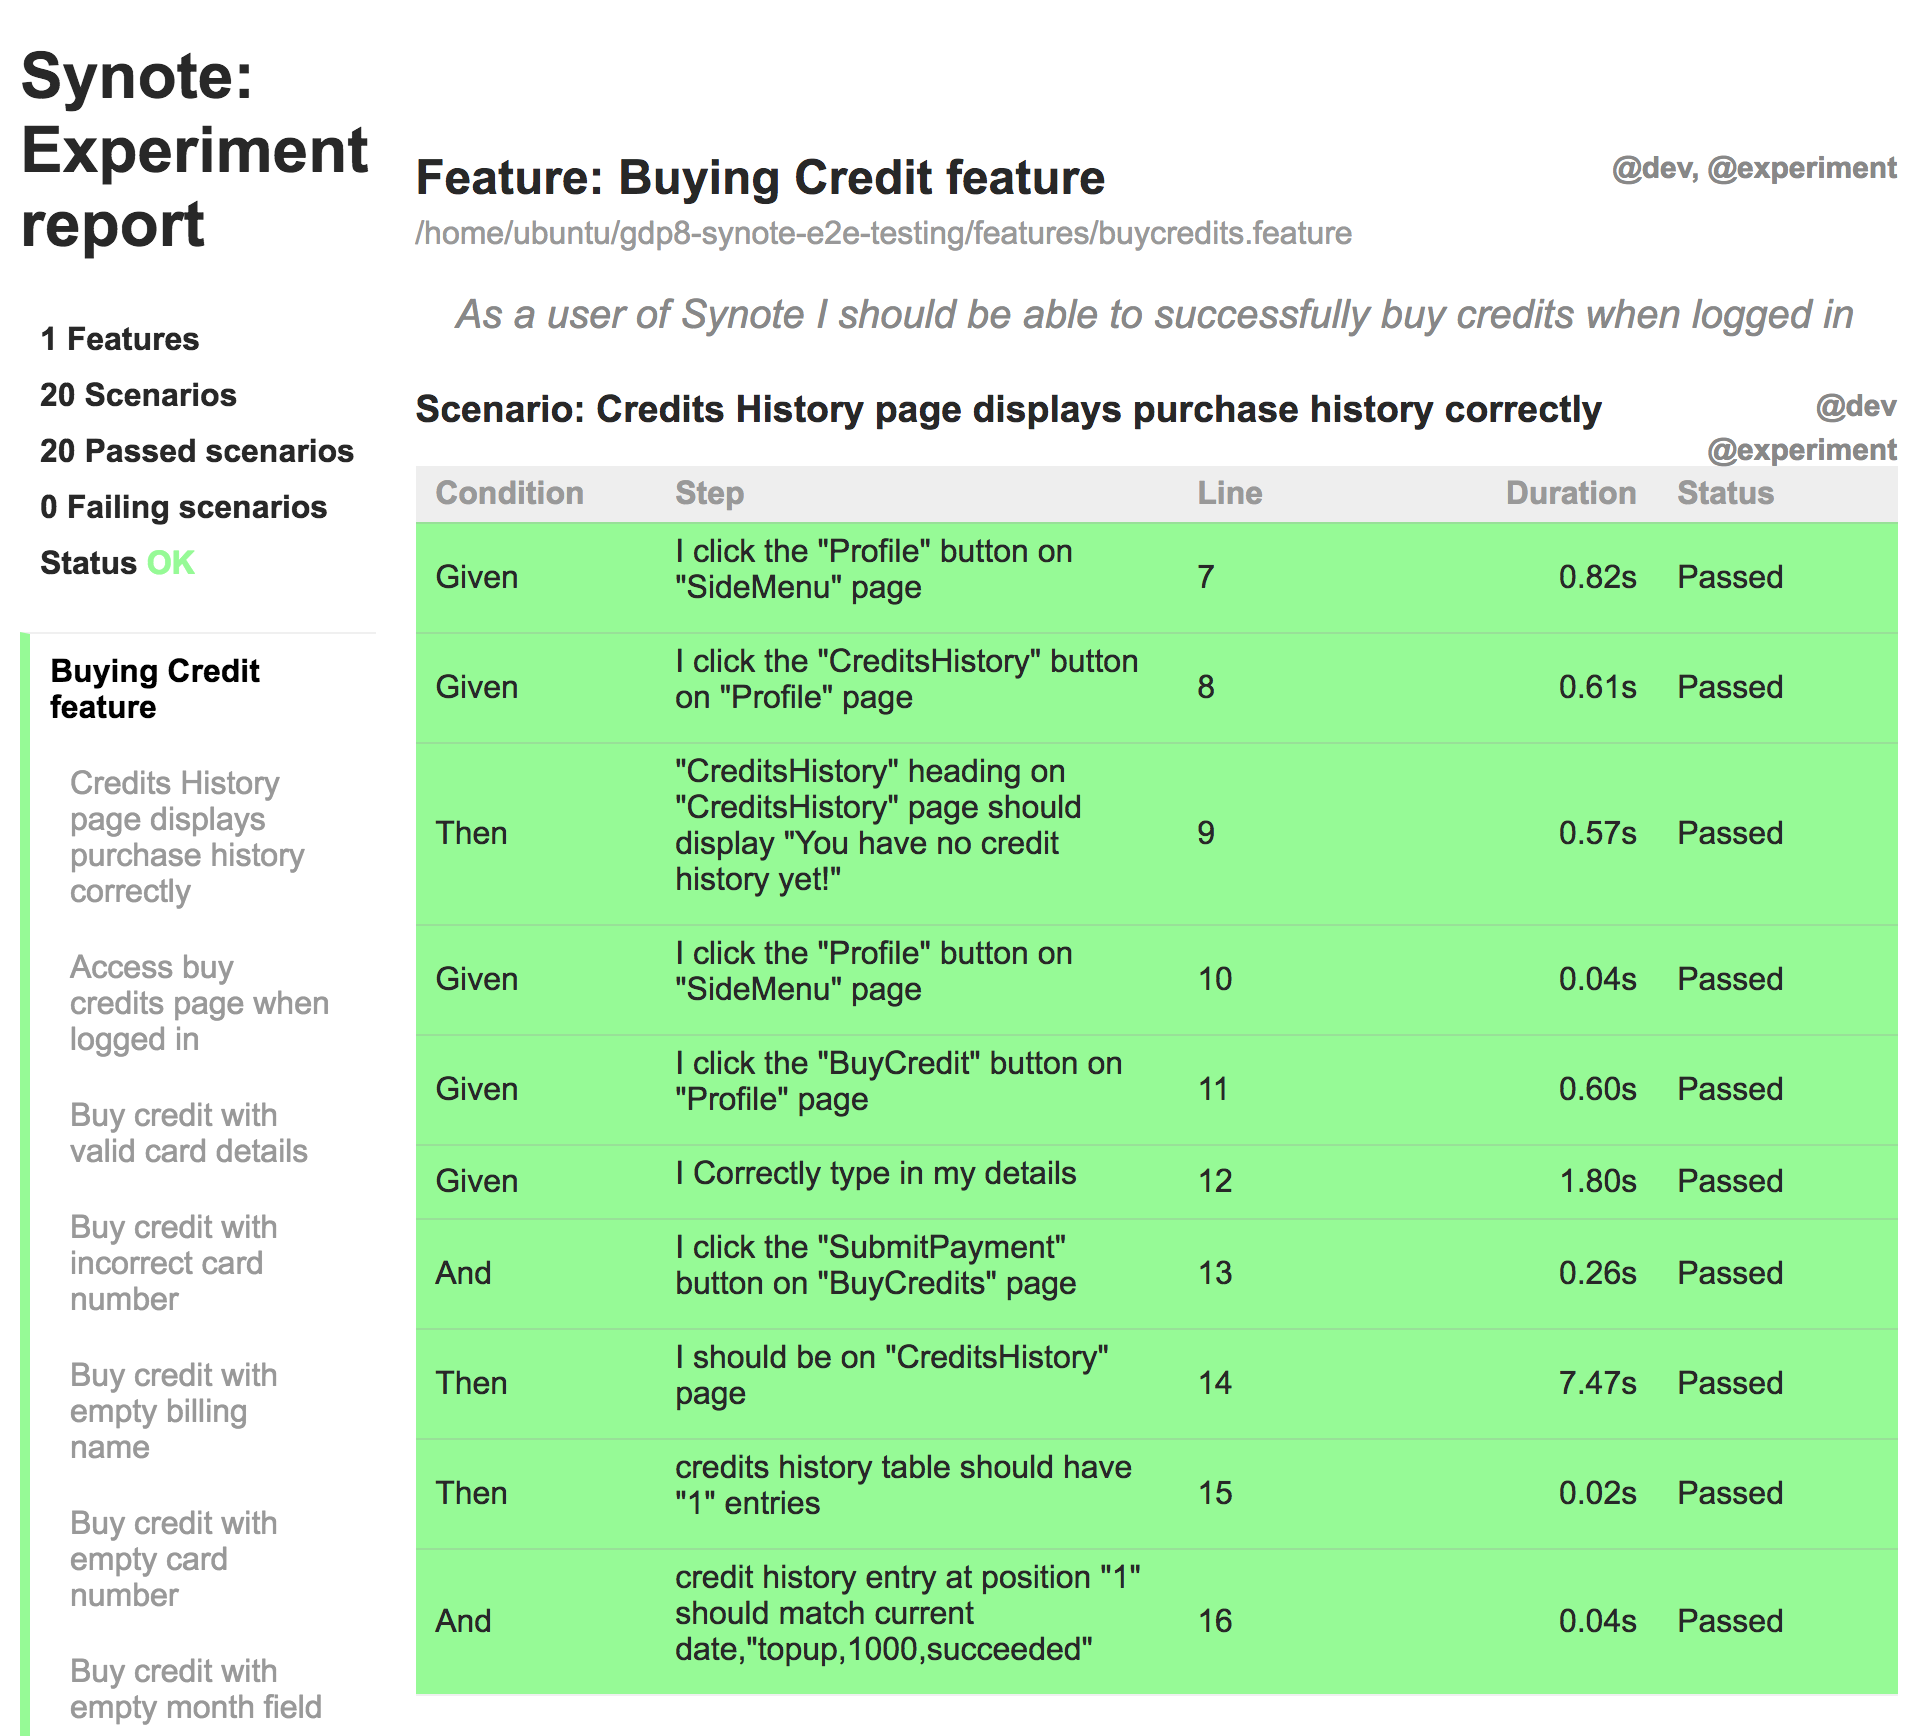
\includegraphics[width=\textwidth]{html-report-example}
  	\caption{HTML Report Example}
 	\label{fig:html-report-example}
\end{figure}

\subsubsection{Reporting Convention}
\label{subsubsec:reporting-convention}

After a number of application builds and subsequent E2E test runs, there will be plenty of reports that stack up. A convention is needed for making sense of these, organising them and linking them with application builds.
\\

All test reports are stored under the \texttt{/reports} folder. There we have separate directories for each Synote site the framework was run against.
\\

One level underneath, we have folders that map to a particular version of the application (latest commit hash). This makes it easier to debug issues and it allows for a critical comparison between versions of Synote. If, for example, a change breaks a large number of tests, the knowledge of the git commit hashes allows us to rollback to a more stable version.
\\

In every hash commit folder, we have one or more directories whose names represent timestamps as year-month-day\_hour-minute-second. Finally, in each timestamp folder we have the actual test report in HTML and JSON format along with screenshots of the failed tests. An example overview of this convention can be seen in \textbf{Figure \ref{fig:reports-file-structure}}.
\\

\dirtree{%
  .1 reports/.
  .2 experiment/.
  .3 18cc3efc46dc0185a46315b8e97710c8666057c2.
  .4 2016-12-24\_23-59-59.
  .5 index.html.
  .5 index.json.
  .5 Buy\_credit\_with\_empty\_card\_number\_42.png.
  .2 production/.
  .3 b6bd0be898f0c3285684d3a25a542914840a42ee.
  .4 2016-11-31\_00-00-00.
  .5 index.html.
  .5 index.json.
  .5 Buy\_credit\_with\_invalid\_expiry\_60.png.
  .5 VAT\_will\_be\_added\_at\_20\_when\_buying\_credits\_78.png.
}
\captionof{figure}{Example Reports File Structure}
\label{fig:reports-file-structure}

\subsection{Assessment}
\label{subsec:assessment}

The framework's capabilities were thoroughly tested by Deepak, who wrote most of the test cases. Tom focused on the second iteration of the payment feature and was purposefully not involved in the initial prototyping of the testing framework. This enabled Tom to have an outside perspective of the framework to provide an assessment of its ease of use. Armed with the framework repository and a readme file, Tom set about writing a test for the latest payment feature functionality he had added.\\

Following the readme file, the first step is to install the dependencies. This was the first time the framework had been installed on a Windows machine and due to an installation of Visual Studio, an error occurred. After resolving this issue, the relevant steps were added to the readme and progress resumed. After browsing the existing files relevant to each section in the readme, it was apparent that nearly all the tools Tom needed existed already. Lines 1-3 \& 5 of \textbf{Listing \ref{lst:toms-first-test}} make use of existing step methods. However, line 4 required an extension of the existing method in \textbf{Listing \ref{lst:buycredits-step-file}} to allow repeated clicks as shown in \textbf{Listing \ref{lst:additional-step-method}}.\\

\begin{listing}[H]
\begin{minted}[xleftmargin=\parindent, linenos, breaklines, breakanywhere, bgcolor=lightgray, fontsize=\small]{cucumber}
Scenario: Maximum purchase cost reached
  Given I click the "Profile" button on "SideMenu" page
  Given I click the "BuyCredit" button on "Profile" page
  Given I click the "IncrementCredit" button on "BuyCredits" page 59 times
  Then Increment credit button should be disabled
\end{minted}
\captionof{listing}{Tom's First Test}
\label{lst:toms-first-test}
\end{listing}

\begin{listing}[H]
\begin{minted}[xleftmargin=\parindent, linenos, breaklines, breakanywhere, bgcolor=lightgray, fontsize=\small]{js}
this.Given(/^I click the "([^"]*)" button on "([^"]*)" page (\d+) times$/,
  function (buttonName, pageName, times) {
    var promises = [];
    for(var i = 0; i < times; i++) {
      promises.push(this.Support.clickButton(buttonName, pageName));
    }
    return Promise.all(promises);
});
\end{minted}
\captionof{listing}{Additional Step Method}
\label{lst:additional-step-method}
\end{listing}

Again, referring to the readme file, Tom ran the test suite on his local development machine and watched as the test he had written passed first time. As this was local testing, the actions were executed in a browser window providing visual confirmation that the desired actions were performed. Thus, with no prior knowledge, Tom was able to use the framework to write and execute a successful E2E test.
